\documentclass[12pt]{article}

\usepackage{fullpage}
\usepackage{graphicx, rotating, booktabs} 
\usepackage{times} 
\usepackage{fbb} 
\usepackage{natbib} 
\usepackage{indentfirst} 
\usepackage{setspace}
\usepackage{grffile} 
\usepackage{hyperref}
\usepackage{tikz}
\usepackage[export]{adjustbox}
\usepackage[most]{tcolorbox}
\usepackage{verbatimbox}
\usepackage{lscape}
\usepackage{afterpage}
\usepackage{amsmath}
\usepackage[labelfont={bf},textfont=it,labelsep=period]{caption}
 \usepackage{multirow} 
\setcitestyle{aysep{}}
\usepackage{dcolumn}

\hypersetup{
  colorlinks = true,
  urlcolor = blue,
  linkcolor = black,
  citecolor = black,
  pdfauthor = {Joshua Alley},
  pdfkeywords = {},
  pdftitle = {},
  pdfsubject = {},
  pdfpagemode = UseNone,
%  pdffitwindow = true
%  pdfcenterwindow = true
}



\singlespace
\title{\textbf{Economic Bargaining in Asymmetric Alliances}}
\author{
Joshua Alley\\
Postdoctoral Research Associate\\
Democratic Statecraft Lab\\
University of Virginia 
}
 
\date{\today}

\bibliographystyle{apsr}

\usepackage{sectsty}
\sectionfont{\Large}
\subsectionfont{\noindent\large\textit}
\subsubsectionfont{\normalsize}

\makeatletter
\renewcommand\tiny{\@setfontsize\tiny{9}{10}}
\makeatother


\begin{document}

\maketitle 

\begin{abstract}
Can military alliance leaders leverage their preponderant security role to extract economic concessions from junior partners?
Some argue that powerful states can manipulate the extent of their security commitments to coerce economic changes. 
Others believe that large states place too much value of security ties to exert economic leverage.  
I argue that junior alliance members will only make temporary economic concessions to support committed allied leaders' tenure in office. 
I test these claims with a analyses of exports from democratic major powers to their proteges and U.S. exports to allies. 
I find that prior leader signals of commitment increase exports to allied states during election years. 
An analysis of exports from U.S. states shows that exports from swing states to allies increase more than exports from other states. 
These results suggest that leaders can leverage security ties for temporary economic and political gain by encouraging allies to back their efforts to remain in office, but doing so requires consistent commitment signals. 
\end{abstract} 


\newpage 
\doublespace 


\section{Introduction}

%In 2018, a former Obama administration official argued that ``"Trump is trying to conflate his issues over trade and his beef with Europe and the EU with NATO, and he's using our military strength to do that.''\footnote{\url{https://www.usatoday.com/story/news/politics/2018/07/11/donald-trump-complains-trade-europe-nato-summit/774495002/}}
In 2019, when Donald Trump argued that ``It's not right to be taken advantage of on NATO and also then to be taken advantage of on trade, and that's what happens,'' he was not the first or last U.S. policymaker to highlight perceived problematic economic concessions to U.S. allies.
Then Secretary of the Treasury John Connally claimed in a 1971 speech that the United States ``had the right to expect more equitable trading arrangements'' with its allies (quoted in \citep[pg 175]{Sayle2019}).
%\footnote{See also: \url{https://www.fpri.org/article/2019/04/the-blue-chip-and-the-little-blue-bird-change-and-continuity-in-nato-policy-from-nixon-to-trump/} and \url{https://history.state.gov/historicaldocuments/frus1969-76v03/d155}}
More recently, some leading congressmen criticized the Biden administration's decision to waive sanctions on the Nord Stream 2 gas pipeline between Russia and Germany.\footnote{\url{https://www.bbc.com/news/world-us-canada-57180674}}


These examples reflect a general question; can large alliance leaders leverage their preponderant security role for economic influence over junior allies? 
There are two schools of thought on economic bargaining in asymmetric alliances. 
One argues that because leading states prioritize geopolitical aims, they have limited economic leverage \citep{Drezner2013, WolfordKim2017}.
Another perspective argues that threatening to manipulate security commitments encourages economic concessions \citep[pg. 122]{Oatley2015}. 


I argue that the economic leverage of large alliance members depends on potential leadership changes and past efforts to reassure allies.
Whether leaders reassure allies through public statements and tolerating trade competition determines their subsequent leverage when they seek economic concessions in support of their efforts to remain in office. 
Small allies will be more likely to make economic concessions if they can help a committed partner retain power without endangering their own tenure in office.  
Thus, leaders who have previously demonstrated commitment to an alliance are more likely to secure economic concessions, but those concessions will often be temporary and targeted, rather than structural.
Senior allies thus have little economic leverage, unless potential leadership change encourages their partners to make economic concessions as temporary expedients to bolster their long-run security. 


% Findings


% economic and seucrity ties 
The argument and findings address three salient issues in international relations theory and practice. 
First, they speak to debates about the connection between economic and security ties \citep{Mastanduno2009, Poast2019}. 
Scholars disputed whether economic linkages drive security ties \citep{BiglaiserDeRouen2007, Fordham2010, Kimball2010}, security concerns encourage economic linkages \citep{Gowa1995, Li2003, LongLeeds2006, GowaMansfield2004}, or the relationship goes in both directions \citep{BiglaiserDeRouen2009, KinneBunte2018}. 
I find that security concerns shape economic links most of the time, but the relationship flips when states use economic policy to cement security relationships.


% economic cycles
Expanded exports from alliance leaders to junior partners in election years could also be part of a political business cycles where elites manipulate economic policy to increase their odds of reelection. 
Elected leaders often use fiscal \citep{Rogoff1987} and monetary policy \citep{ClarkHallerberg2000} to generate economic growth around elections. 
There is also evidence that leaders use non-budget instruments like social policy \citep{Philips2020}, social pacts with unions \citep{Ahlquist2010}, trade disputes \citep{Conconietal2017} and defense contracts \citep{DerouenHeo2000} to bolster their electoral prospects. 
I find that allies contribute to political business cycles when the incumbent leader has backed their security interests.



% coercion
Finally, this paper provides new insight into coercive demands by bridging economic and security bargaining.
When and why coercion succeeds is an important question \citep{Sechser2010, Sechser2018, Cebuletal2021}.  
Most studies of coercion examine either security threats (e.g. \citep{HorowitzReiter2001, Sechser2011}) or economic sanctions (e.g. \citep{Marinov2005, Allen2008, Escriba-FolchWright2010}).
This study explores whether security ties provide economic leverage. 
In particular, it explores issue linkage as part of alliance management, building on previous work that considers alliance formation \citep{Poast2012} and credibility \citep{Davis2008, Poast2013}. 


% policy 
Whether trade concessions are the price of security alliances also has important implications for how policymakers bargain with allies. 
If threats to reduce security commitments does not lead to economic concessions, then they create negative security consequences without corresponding economic gains for either party. 


\section{Argument}


%Whether large alliance members can coerce economic change in smaller allies also adds a new dimension to our understanding of coercion. 
%Classic studies of coercion with security threats often focus on security outcomes in a crisis bargaining framework \citep{Sechser2011, Cebuletal2021}. 
%Other studies of economic coercion through sanctions considers political \citep{Marinov2005, Bapatetal2016} and economic aims. 
%This study examines how security threats shape economic ties. 
%Prior scholarship on gunboat diplomacy and trade is the most closely related work in prior scholarship. 
%\autoref{tab:sec-econ-coerce} summarizes the place of this work in studies of coercion.
%
%
%
%\begin{table}[hbt!]
%\begin{center}
%\begin{tabular}{| p{0.2\linewidth} | p{0.4\linewidth} | p{0.4\linewidth} | }
%\hline
%              &   Security Threat & Economic Threat \\
%\hline                  
%Security Demand  & Crisis Bargaining &  Sanctions for Political Change \\
%Economic Demand  & \textbf{Economic Bargaining Between Allies}, Gunboat Diplomacy  &  Sanctions for Political Change  \\     
%\hline                          
%\end{tabular}
%\caption{Potential threats and aims in coercive bargaining.}
%\label{tab:sec-econ-coerce}
%\end{center} 
%\end{table}


% basic asymm alliance framework
This argument considers economic bargaining in asymmetric alliances. 
In alliances between large and small states, the large state protects its junior partner in exchange for foreign policy concessions \citep{Morrow1991}.
As part of this bargain, alliance leaders often tolerate economic protectionism by allies \citep{Mastanduno1998, WolfordKim2017}. 


Military alliances are connected to economic cooperation.
Conflict and economic integration are inseparable (see for example, \citep{GartzkeLi2003, Chen2021}).
Many alliances also include explicit or implicit linkages to economic cooperation \citep{LongLeeds2006, Davis2008, Poast2012}. 


In a similar vein, there are two competing perspectives on the relative bargaining leverage of large and small members in asymmetric alliances.
One argues that to prioritize international influence and geopolitical concerns, large states tolerate economic protectionism and inefficiencies by allies, leaving them little economic leverage \citep{Drezner2013, WolfordKim2017}. 
Another view claims that threats to reduce commitment can coerce economic concessions from junior alliance partners \citep{Oatley2015}.  


% overview
I argue that the relationship between security from alliances and economic bargaining depends on leadership cycles in the large alliance partner.  
Only leaders that have established a reputation for cooperation with allies can leverage their security commitments for economic concessions. 
Those concessions are often temporary rather than structural, as allies attempt to support a friendly leader without endangering their own security in office. 


% actors 
There are four key actors in this argument. 
First, a leader in the large alliance member seeks geopolitical influence and a favorable balance of economic relations. 
A leader in the small alliance member seeks security from external threat and a favorable economic balance.
Both sets of leaders are office-seeking, and depend on domestic support to stay in power.
Domestic actors in both states can gain or lose from changes in economic ties between the allied states. 


% issue- must keep domestic actors happy to retain power
Leaders in the small and large alliance members must retain adequate domestic support to continue in office. 
Assuming incomplete trade openness, some domestic sectors in both states are protected from foreign trade competition by tariff or non-tariff barriers. 
The large state has greater market power in international trade. 


% distributional consequences
Economic barriers have distributional consequences for domestic interests in large and small alliance members.
Keeping out exports increases the income of protected sectors in the junior alliance member that would otherwise have to compete with exports from the large state.
Concessions to a large ally would reduce their income, which would likely reduce their support for the incumbent leader, as trade cleavages shape domestic political coalitions \citep{Rogowski1987, Hiscox2001}. 


% response: lean on allies for concessions, especially when there's a risk of losing office
At the same time, liberalization would benefit large allied exporters by increasing their market share, which creates a domestic political motive for large states to renegotiate the balance of economic and security relations in an alliance. 
Economic concessions could benefit domestic interests, large alliance member leaders could place economic pressure on their allies to bolster their political position. 
Leaders will thus be especially inclined to seek a more favorable alliance arrangement when they risk losing office through an election or some other leadership challenge. 


% exact threat 
Threatening to reconsider their security commitments to smaller partners is one way for large state economic leaders can seek economic concessions.
At bottom, these threats are motivated by electoral considerations--- a sense that allied economic policies affect prosperity and leadership competition. 
Given leadership competition, these demands contain an implicit threat that failing to concede might endanger security cooperation by empowering a less committed leader.


% allied incentives to concede- want to keep security, must keep their interests happy too
% new leader might be similar, but less certainty. 
When the large state leader makes a security threat for economic concessions, they create a dilemma for small alliance members. 
Reduced or altered security commitments endanger small state security, but economic concessions threaten a leader's hold on office by harming domestic interests. 
Small state leaders thus weigh the likely security benefits of conceding with the domestic political consequences of economic concessions.


% only concede if enough prior res: cooperative reputation
The leaders of a small alliance member will only make economic concessions if they believe that supporting the efforts of the large alliance leader to retain power offers sufficient security benefits. 
Economic concessions thus depend on the large state leader's reputation for cooperation. 
If the large state leader has demonstrated strong commitment to the alliance before making economic demands, then adjusting economic relations to help them retain power is worthwhile, as it promotes future security cooperation. 
The leadership challenger in the large state might be less committed, and small state leaders would prefer a known favorable partner to the uncertainty of a leadership change, given the high stakes of changes in alliance commitments.


% prior res establishes rep for restraint too: cebul et al
In addition to establishing that concessions will bolster long-run security by helping a friendly leader remain in office, a prior cooperative reputation establishes a necessary reputation for restraint. 
Committing to not renege and follow through on a threat regardless of cooperation is essential in coercive bargaining \citep{Cebuletal2021}. 
If a leader has previously demonstrated commitment to the alliance, it reduces the perceived risk that they will demand further concessions, or reduce security commitment regardless.
This decreases the likelihood of small states attempting to establish a reputation for resolve to ward off future challenges, which makes coercive failure more likely \citep{Sechser2010, Sechser2018}. 


% Indicators: prior tolerance of allied protectionism, statements
In economic bargaining between allies, reputations for commitment adhere to leaders, who have substantial influence on foreign and economic policy \citep{Renshonetal2018}.
Statements of reassurance and commitment to an alliance are one salient way for leaders to establish a cooperative reputation \citep{Blankenship2020}.
Prior tolerance for allied protectionism and deference to allied economic interests is another indicator of cooperation by large state leaders.
Bearing the costs of allied economic actions is a costly signal of commitment to an alliance because it has economic consequences. 
Thus, leaders who support allies early in their tenure establish a cooperative reputation that encourages junior allies to make economic concessions when they face leadership challenges.


% don't concede too much, however
Even when a leader has a cooperative reputation, domestic concerns constrain allied economic concessions \citep{Davis2008}. 
Reducing protection for domestic industries exposes a leader to domestic political pressure. 
Taking down trade barriers is also hard to reverse, especially when states are part of international organizations.
Structural changes increase the risk of a small state leader losing office.  
The result is that small states will make temporary concessions to help cooperative leaders remain in office, while avoiding structural changes. 
Symbolic, temporary and targeted measures can give a large state incumbent a competitive boost without antagonizing domestic interests. 
Large states can therefore only leverage their preponderant security role in specific and limited ways.


% Govt purchases to address BoP and trade deficit. 
Government purchases are the most likely concession by small allies. 
These purchases can address large allied concerns with trade deficits and the balance of payments without reducing trade protection for domestic interests. 
For example, \citep{Bergeretal2013} find that CIA interventions increased U.S. exports to targeted countries via government purchases.


% Might even be targeted by region. 
Moreover, purchases can address the political competition concerns of large state leaders.
Perhaps small states could target their purchases in crucial electoral districts to bolster a cooperative democratic leader, for instance. 
In autocracies, purchases could favor members of the leaders' winning coalition, whether by geography or sector.


% explains a couple recent things- illustrative
% why'd Biden concede on Nord stream 2? 
Several recent interactions between the United States and its allies help illustrate the argument. 
First, the Biden administration's controversial decision to waive sanctions and allow completion of the Nord Stream 2 gas pipeline between Germany and Russia is likely part of the Biden administration's efforts to reassure European allies. 
In addition to allowing this concession to German economic concerns, Biden sought to wind down many of Trump's European trade disputes while talking up the U.S. commitment to NATO and the EU.\footnote{\url{https://www.aljazeera.com/economy/2021/6/15/eu-and-us-call-truce-in-trump-era-trade-war}}


% why did Trump fail to get substantial economic concessions from allies? 
The argument also explains why U.S. allies rarely conceded Donald Trump's trade demands. 
Trump's prior rhetorical attacks on NATO and other U.S. alliances gave allies few incentives help him win re-election. 
Economic concessions might have aided Trump's re-election campaign, just as Chinese tariffs on soy reduced Republican's vote share in the 2018 election \citep{ChyzhUrbatsch2021}. 
Moreover, Trump sought fundamental alterations to trade policy such as reduced barriers to U.S. agricultural products that might have endangered allied leaders' political survival \citep{HeeParkJensen2007}.



\subsection{Implications}



This argument has several testable implications, especially for democratic alliance leaders.
Elections provide clear indicators of when a leader might be replaced. 
This also facilitates strategic anticipation on the part of allies and leaders, who can adjust their economic bargaining accordingly. 
The relatively open nature of electoral competition also facilitates potential allied influence. 


The first prediction is that economic pressure from larger allies will be more likely when the leader faces replacement through election or some other competition. 
Given pressure to deliver for domestic interests to remain in office, leaders will be more likely to make economic demands of allies when there is a high chance they will be replaced. 
These demands are especially likely to cover issues with distributional consequences like trade.


\begin{quote}
\textsc{Economic Demands Hypothesis: As the likelihood of a leadership change increases, leaders of large alliance members will make more economic demands of allies.}
\end{quote}


The second hypothesis concerns whether junior partners make economic concessions. 
Junior partners will increase their imports from allies when the leader facing replacement has demonstrated prior commitment to the alliance. 
Otherwise, junior alliance members may take a chance on elections empowering a more supportive leader. 
Past indicators of commitment include statements of reassurance \citep{Blankenship2020} and trade concessions \citep{WolfordKim2017}.


\begin{quote}
\textsc{Economic Concession Hypothesis: When the leader of a large alliance member might be replaced, imports from junior allies will increase as prior commitment signals by that leader increase.}
\end{quote}



The final hypothesis predicts targeted concessions.
If allies want to support a friendly leader, they may target their economic concessions to crucial regions of electoral contests. 
In the United States, swing states have a critical role in presidential elections, which encourages U.S. leaders to target them in economic policies like WTO disputes \citep{Conconietal2017}.
Therefore, one potential implication is that exports from swing states to U.S. allies will increase in the year of elections as the incumbent's reputation for alliance commitment increases.

\begin{quote}
\textsc{Swing States Hypothesis: In the year before and year of presidential elections, exports from swing states to U.S. allies will increases as the number of prior reassurance statements by the incumbent President increases.}
\end{quote}



\subsection{Objections and Alternative Explanations}


% objection- why not dismiss threats/demands by committed leaders as incredible? 
% stand to benefit from helping them
Before proceeding to how I test these hypotheses, I consider several potential objections and alternatives to the argument, including whether committed leaders can make credible economic demands and the role of external threat.
First, why do junior partners to concede economic demands to committed leaders? 
While government purchases are less consequential than tariff changes, spending funds on U.S. exports still imposes opportunity costs.
I expect that purchases are worthwhile to support the security benefits of a committed allied leader. 
Conceding purchases greater security in expectation. 


% threat: increases sec demand, but makes it harder to walk away for large partner
% Cold War should make that fairly clear. 
Another objection is that increased external threat might make junior alliance partners more receptive to economic demands from their patron.
Conceding to ensure protection might be worthwhile, in short.
Though this is plausible, it ignores the incentives of the large partner, who also has more to lose from weakening an alliance if the threat to junior partners is greater. 
Cold War dynamics illustrate this issue.
Although the United States initially tolerated and even encouraged European and Japanese protectionism to ensure that allies could rebuild their economies and military capabilities, later efforts to negotiate more favorable trade terms led to substantial resistance from the U.S. security establishment who feared that U.S. economic nationalism would increase Soviet influence \citep{Mastanduno1998}.
Threats place pressure on both alliance parties, albeit on different margins.


In the following, I describe how I test each of these hypotheses. 
In the first analysis, I establish that more committed leaders of major powers receive greater exports from their allies in election years. 
The second analysis shows that increasing U.S. exports to allied states in election years are concentrated in swing states, which suggests allied concessions concentrate in key electoral constituencies.




\section{Economic Demands by Large Allies (Placeholder for H1)}




\section{Democratic Major Power Exports to Allies}

To test the economic concession hypothesis, I analyze exports from major powers to their allies. 
I expect that when an election could replace leaders who have made more prior signals of commitment to their alliance partners, exports from that state to allies will increase. 
In non-election years, signals of support will reduce economic leverage over allies.
This implies a positive interaction term between leader support and election year variables, and a null or negative constituent term on the leader signals of support measure.


The outcome of interest is the log of annual exports from democratic major powers to their proteges. 
This dyadic dataset includes the United Kingdom, France and the United States and their allies from 1950 to 2012.\footnote{The analysis stops in 2012 due to limits on the major power support measure. I classify France and the UK as junior partners of the United States.}
I draw on exports and imports data from \citep{Barbierietal2009td}.\footnote{Dyadic data from the \textit{peacesciencer} \textsf{R} package \citep{peacesciencer-package}.}


I measure leader commitment to each of these states' allies using the latent measure of \citet{McManusNieman2019}.
Because reputations adhere to leaders, I measure commitment as the moving average of support across the leader's tenure between, using elections data from the National Elections across Democracy and Autocracy (NELDA) dataset \citep{HydeMarinov2012} to identify election years.
I then interact the moving average of protege support with a dummy indicator of election years. 


In addition to the interaction of elections and leader support for allies, I include a series of control variables that may be correlated with alliances and exports. 
The most important control is the lagged log of exports to address temporal autocorrelation in trade ties.
I also adjust for lagged imports, minimum and capital distance between the two states, the GDP of both states \citep{Andersetal2020}, democracy \citep{Marquez2016}, the presence of a militarized interstate dispute \citep{Gibleretal2016} shared IGO membership \citep{Pevehouseetal2020}, lagged or lead election years, and whether an incumbent leader is running. 



Dyadic data is clustered, which can generate misleading regression estimates.
Because major power elections affect multiple dyads, I employ the cluster--robust sandwich estimator of \citep{Aronowetal2015}.
I draw similar conclusions about the conditional relationship between 


I also undertake several robustness checks of the baseline model specification.
The first includes dyad fixed effects in models of changes in exports as a robustness check.\footnote{Fixed effects in dynamic models lead to biased estimates \citep{Nickell1981}.}
I also model dyadic trade balances, transformed with an inverse hyperbolic sine to reduce the impact of positive and negative outliers.
Both these alternative approaches produce similar inferences.


\subsection{Results}

I find that as prior signals of support by a major power leader increase, their exports to allies in election years also increase. 
\autoref{fig:mp-model-coefs} presents the coefficient estimates from the three primary model specifications.
As expected, the interaction between the rolling average of leader's support signals and elections is positive across all three model specifications.


\begin{figure}[htpb]
	\centering
		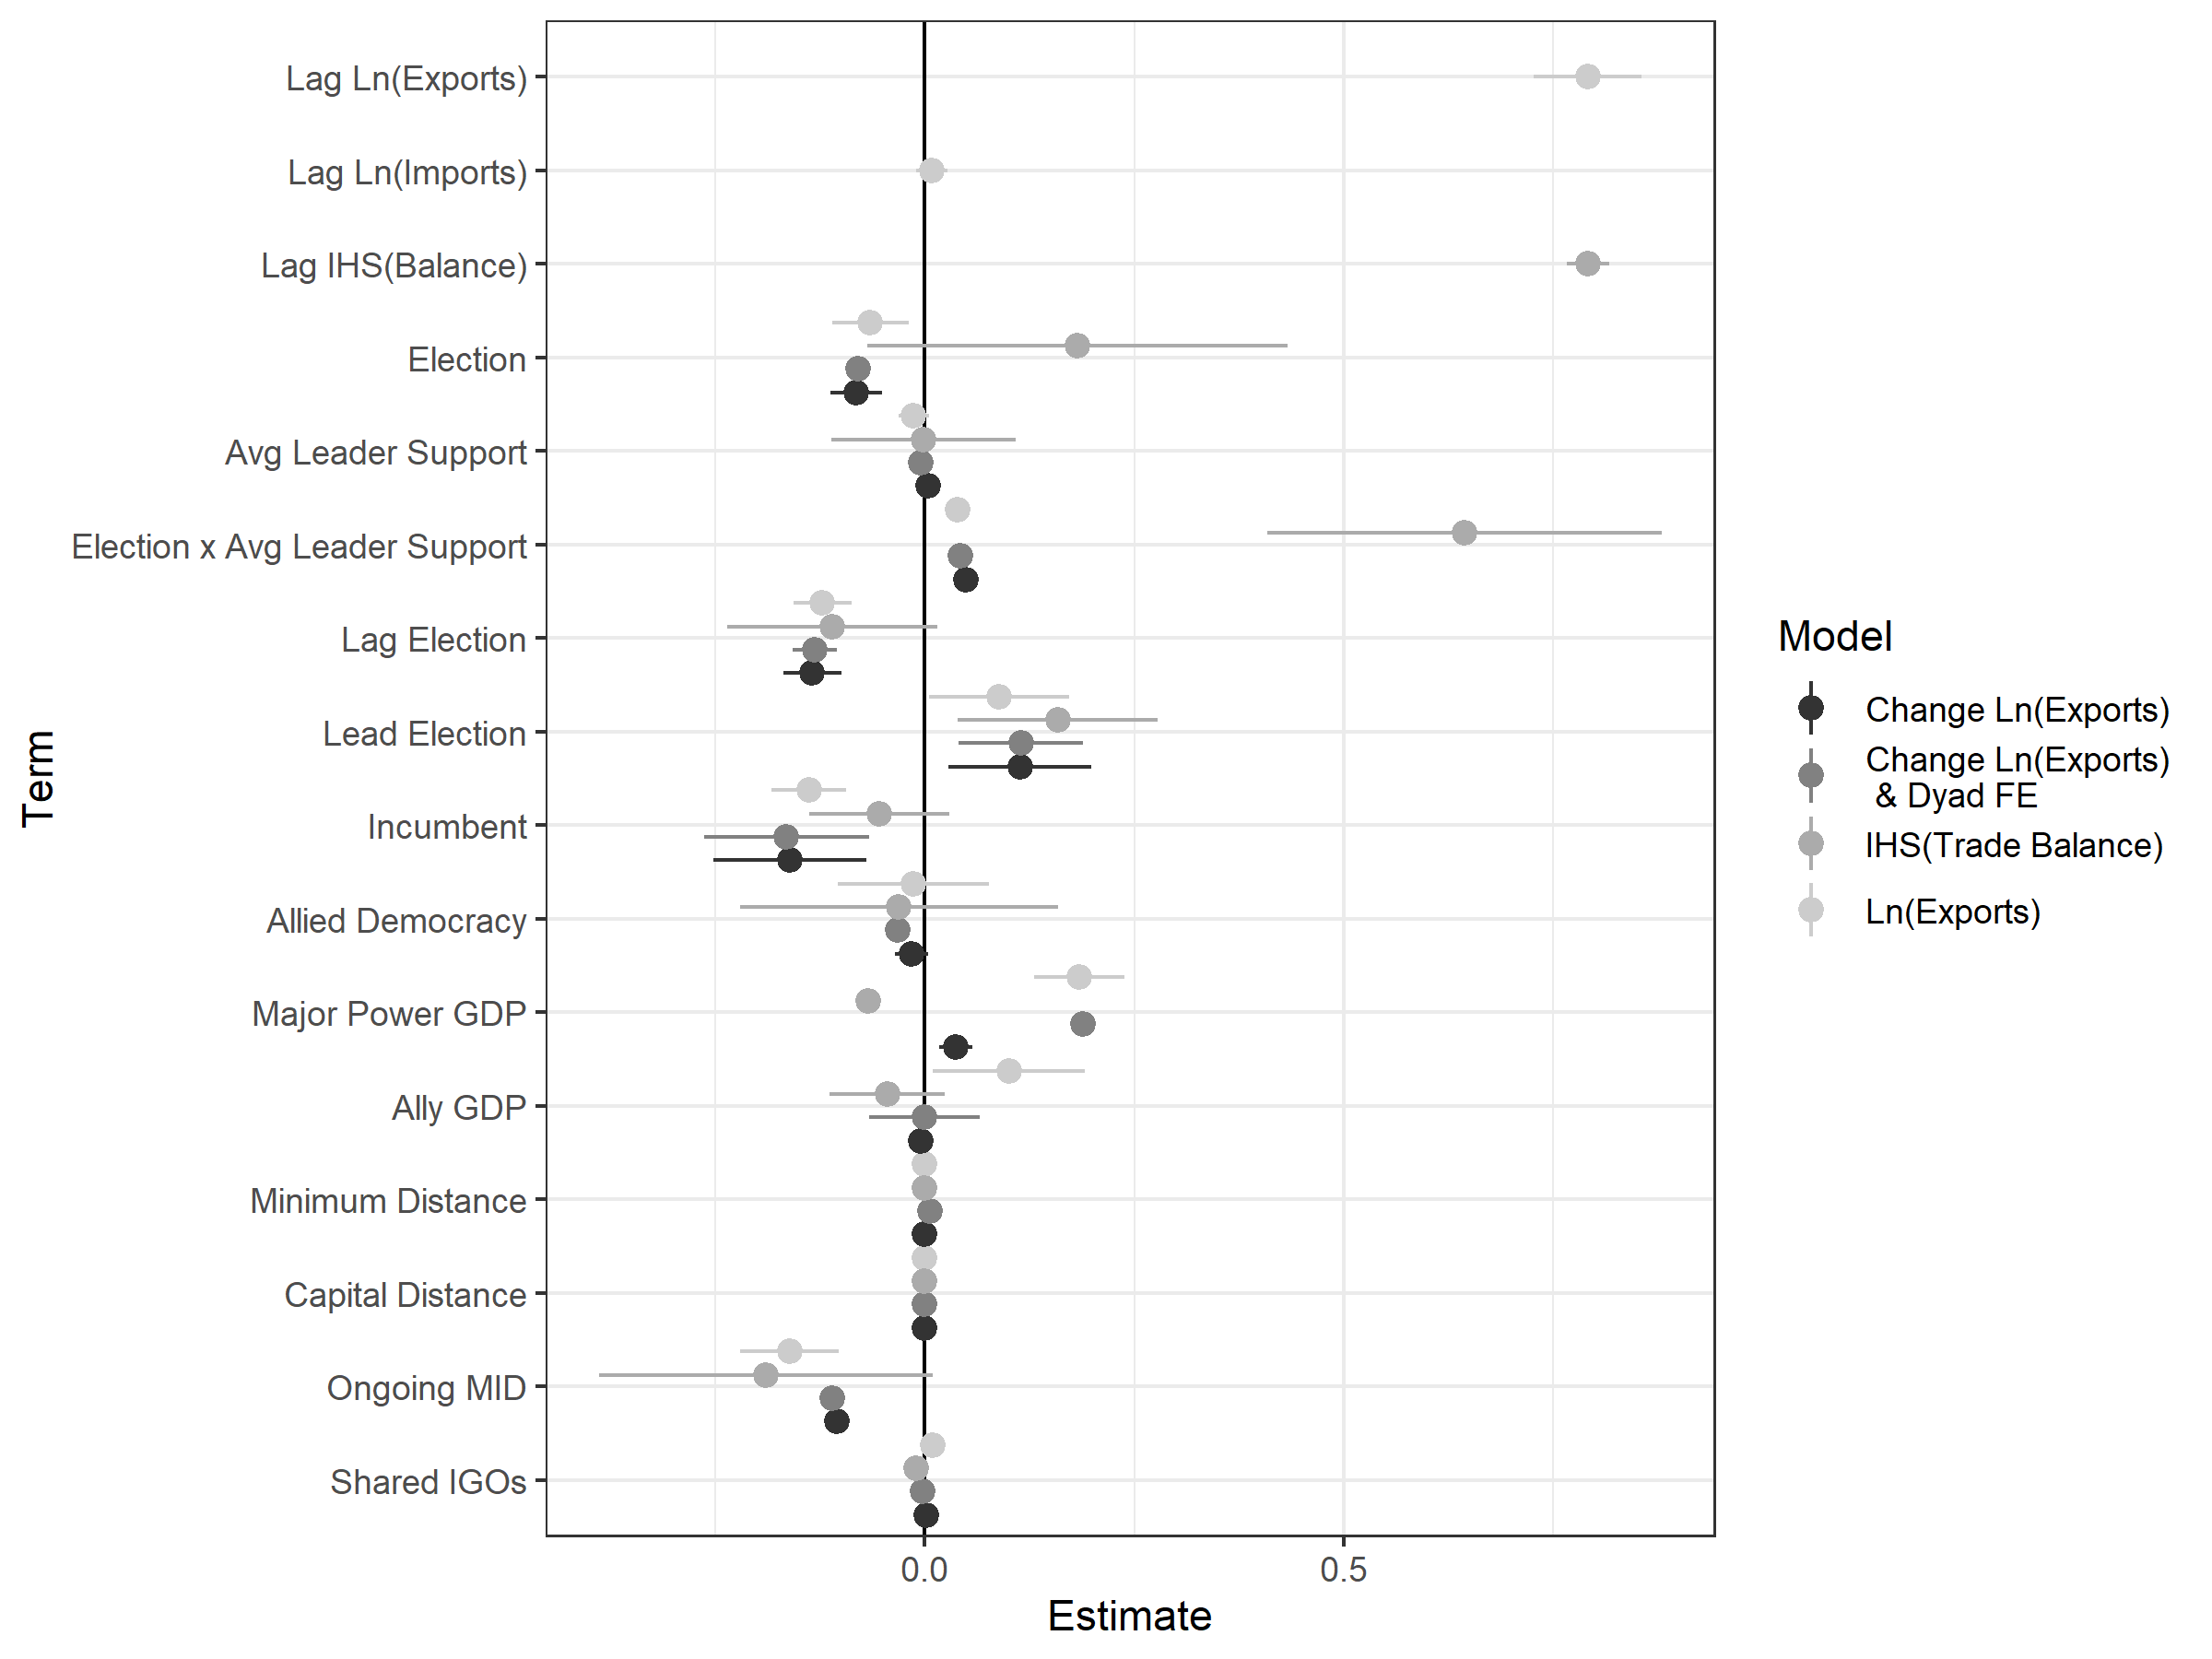
\includegraphics[width=0.95\textwidth]{../figures/mp-model-coefs.png}
	\caption{Coefficient estimates from gravity models of exports from democratic major powers to their junior allies, 1950 to 2012. The first model models annual major power exports and includes a lagged dependent variable. The second model regresses changes in exports on the explanatory variables. The third model examines changes and includes dyadic fixed effects. The fourth model assesses annual trade balances, transformed with an inverse hyperbolic sine. Points mark the coefficient estimate and error bars summarize the 95\% confidence interval.}
	\label{fig:mp-model-coefs}
\end{figure}


The mean leader support constituent term is more mixed.
In years without an election, the association between increasing support signals and exports cannot be differentiated from zero in any of the models and the sign of the estimate shifts with the modeling approach.
Because the election constituent term reflects the impact of an election in years when average leader support is zero and the latent support measure is never equal to zero, that term does not have a similarly straightforward interpretation. 


% control variables show other suggestive evidence of a cycle
Some of the other estimates in \autoref{fig:mp-model-coefs} suggest an electoral cycle in major power exports to their allies.
Exports fall in the year after an election, as the lagged election coefficient suggests.
Exports increase in the year before an election, however. 
Thus, major power exports to allies likely reflect temporary concessions, rather than structural changes.


% marginal effects
The sign and confidence intervals of the interaction terms are inadequate evidence of a conditional relationship \citep{BramborClarkGolder2006}, so I plot marginal effects in \autoref{fig:me-plots-mp}.
This figure presents the estimated marginal effects of increasing average support from a leader in election and non-election years.
In election years, greater prior support from the incumbent leader is positively correlated with major power exports to allies. 
Both the level and annual change in exports are higher for committed leaders in election years.
Outside of election years, the association between prior support and exports could be positive, negative or zero.


\begin{figure}[htpb]
	\centering
		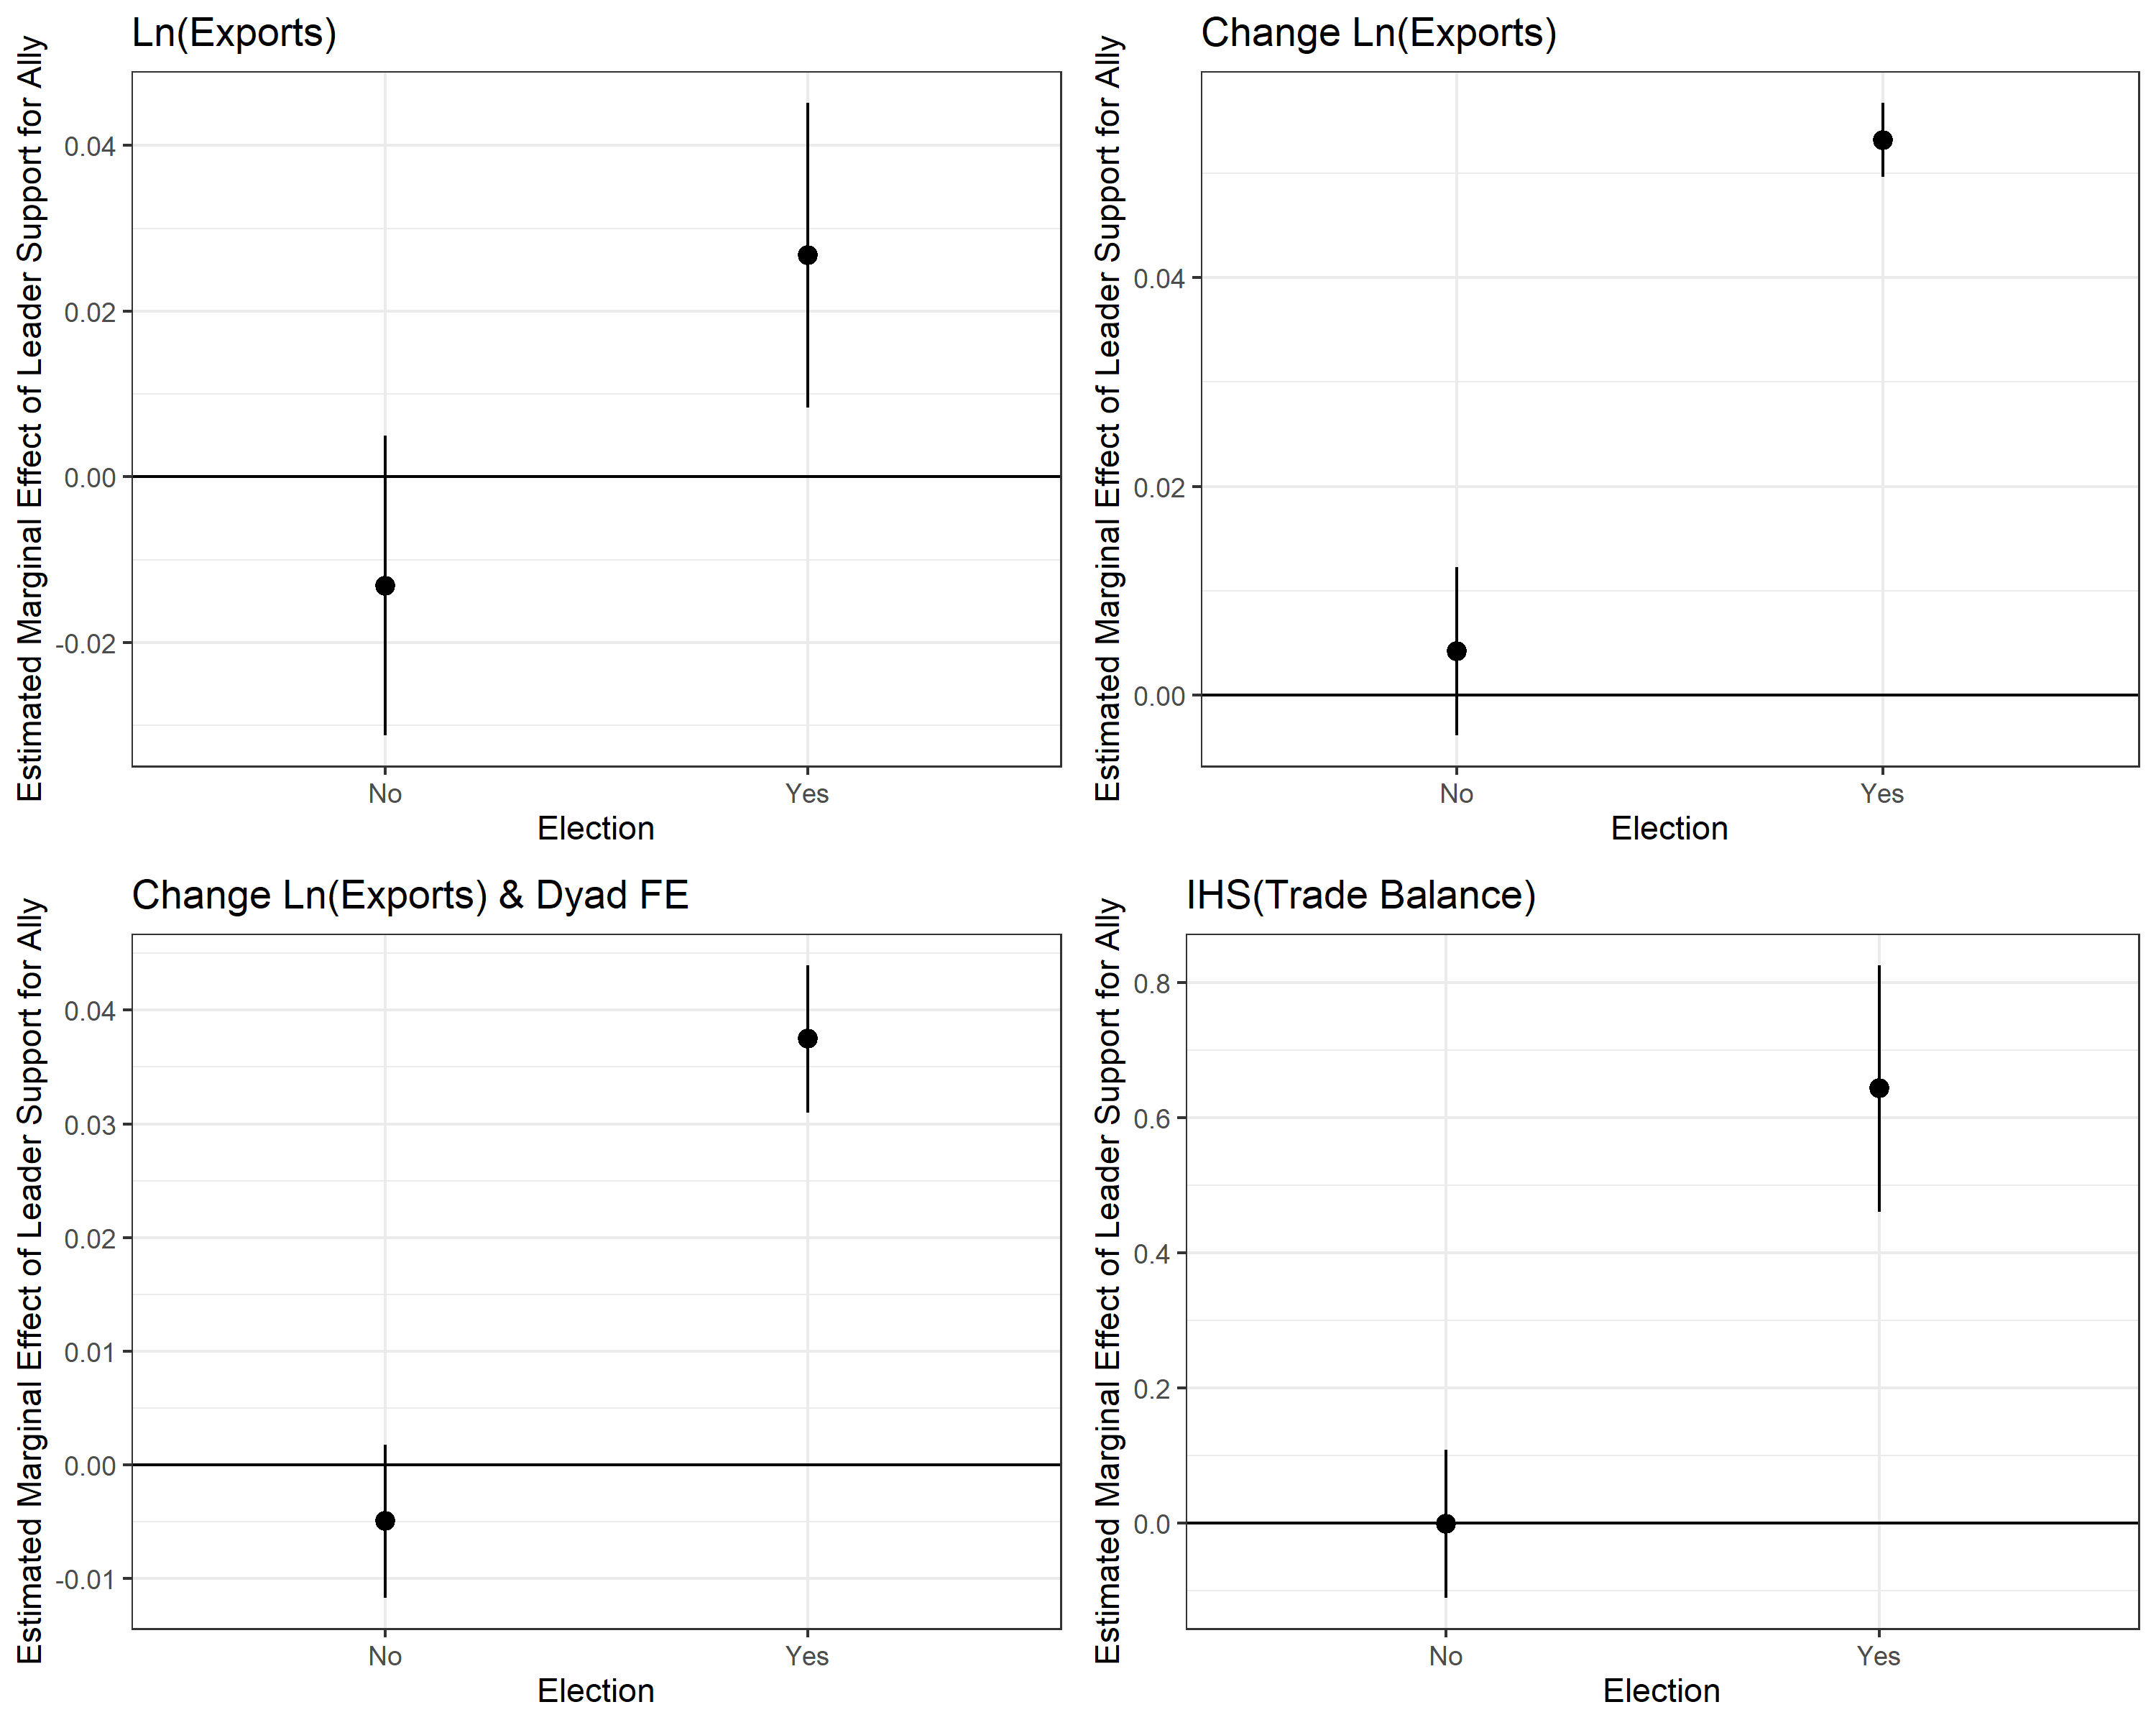
\includegraphics[width=0.95\textwidth]{../figures/me-plots-mp.png}
	\caption{Estimated marginal effect of average signals of support by the incumbent leader on exports from democratic major powers to their junior allies, 1950 to 2012. The first model models annual major power exports and includes a lagged dependent variable. The second model regresses changes in exports on the explanatory variables. The third model examines changes and includes dyadic fixed effects. The fourth model assesses annual trade balances, transformed with an inverse hyperbolic sine. Points mark the coefficient estimate and error bars summarize the 95\% confidence interval.}
	\label{fig:me-plots-mp}
\end{figure}


% improved trade balance
A more positive trade balance follows from allied increases in exports during election years.
Prior signals of support move the trade balance between major powers and their allies in favor of the larger partner during election years, but have no clear impact otherwise.
This is especially salient because leaders often pressure allies for a more favorable trade balance.


These results are consistent with the economic concessions hypothesis. 
When leaders have previously demonstrated commitment to their allies, those allies increase their imports in election years.
In the next analysis, I show that at the least in the U.S. context, these increases in exports are concentrated in electorally competitive states.




\section{Swing States and U.S. Exports to Allies in Election Years}


\subsection{Results}



\singlespace
 
\bibliography{../../MasterBibliography} 


\end{document}